\chapter{Marco Teórico}

En este capítulo se profundizarán los conceptos y conocimientos que sustentan el desarrollo de esta tesis. Fundamentalmente, se explorarán y analizarán los campos y elementos que han sido utilizados directa o indirectamente para el cumplimiento de los objetivos planteados.

Los conceptos presentados a continuación son esenciales para comprender los métodos de compresión y, por ende, para entender el método propuesto en esta investigación. En esta sección se detallarán nociones propias de la teoría de la información desde su paradigma clásico. Posteriormente, a partir de estos conceptos generales, se abordarán las adaptaciones y analogías correspondientes al paradigma de grafos. Estos conceptos son clave para entender la lógica y motivación del algoritmo propuesto, así como para fundamentar las métricas de desempeño que validan el cumplimiento de los objetivos de este trabajo.

\section{Fundamentos de Teoría de la Información}

Al abordar métodos de compresión, es imprescindible partir de ciertos fundamentos esenciales de la teoría de la información. Esta disciplina proporciona el marco matemático necesario para definir, medir y manipular la información contenida en una fuente, y toda técnica de compresión se construye sobre estos principios fundamentales \cite{mackay_nodate, sayood2006introduction}.

El primer concepto clave es el de \textit{auto-información}, que representa la cantidad de información que aporta un evento al ocurrir. Matemáticamente, se define como:

\begin{equation}
i(A) = \log_b \frac{1}{P(A)} = -\log_b P(A)
\end{equation}

Esta expresión refleja la intuición de que un evento raro contiene más información que uno común. El logaritmo actúa de manera inversa a la probabilidad, de modo que cuanto menos probable es un suceso, mayor es su auto-información. En términos intuitivos, se puede pensar que una lluvia en el desierto informa más que una lluvia en una ciudad lluviosa: lo inesperado comunica más \cite{mackay_nodate}.

Cuando la fuente está compuesta por varios eventos posibles $A_i$, cada uno con probabilidad $P(A_i)$, la información promedio que entrega dicha fuente se calcula como una suma ponderada de auto-informaciones, a la que se denomina \textit{entropía}:

\begin{equation}
H = -\sum_i P(A_i) \log_b P(A_i)
\end{equation}

La entropía mide la incertidumbre promedio de la fuente. Shannon demostró que esta cantidad representa el límite inferior teórico del número de bits necesarios para codificar la salida de una fuente sin pérdida \cite{sayood2006introduction, mackay_nodate}. Esto implica que ningún esquema de codificación sin pérdida puede, en promedio, superar la compresión indicada por $H$.

Si se dispone de información adicional sobre el contexto de la fuente, es posible reducir aún más esta incertidumbre. Esta idea se formaliza mediante la \textit{entropía condicional}, que mide la incertidumbre de una variable $X$ dado que se conoce otra variable $Y$ relacionada:

\begin{equation}
H(X|Y) = -\sum_{x,y} P(x, y) \log_b P(x|y)
\end{equation}

Esta medida es particularmente relevante en sistemas predictivos y modelos contextuales, donde la información pasada o contextual ayuda a estimar con mayor certeza la salida futura, resultando en una representación más eficiente \cite{sayood2006introduction}.

A partir de la entropía condicional se define la \textit{información mutua}, que cuantifica la cantidad de incertidumbre que se reduce en una variable $X$ cuando se conoce otra variable $Y$:

\begin{equation}
I(X;Y) = H(X) - H(X|Y)
\end{equation}

La información mutua mide la dependencia o redundancia entre variables, lo que en el contexto de compresión permite aprovechar correlaciones para eliminar duplicidades y reducir la cantidad total de información a representar \cite{mackay_nodate}.

La base del logaritmo en estas definiciones determina la unidad en que se mide la información. En aplicaciones de compresión digital, se usa comúnmente la base 2, dando lugar a unidades en bits, que representan la cantidad mínima de decisiones binarias necesarias para codificar una señal. En contextos más teóricos, también se emplean bases como $e$ (nats) o 10 (hartleys), aunque su uso es menos frecuente en aplicaciones prácticas \cite{sayood2006introduction}.

En resumen, la teoría de la información no solo permite comprender cuánto es posible comprimir una señal sin perder información, sino que también establece límites y directrices para diseñar sistemas de compresión eficientes. La identificación de redundancias, la modelación de fuentes y la toma de decisiones óptimas en codificación descansan sobre estos conceptos fundamentales \cite{sayood2006introduction}.

% EXPLICAR PCAAAAAAA
\section{Transform Based Coding}\label{sec:transform_based_coding}
    La codificación basada en transformadas es un fundamento esencial en el campo de la compresión de datos. Esta detalla la capacidad de una o varias funciones (transformadas) de representar cierto espacio $U$ en otro $V$ donde la concentración de la energía de ciertas características de la señal sea mayor. Estas características se consideran de interés mediante métricas cuantitativas o cualitativas de interés para cada contexto de aplicación.
    \\
    
    
    \subsection{Transformación Lineal}
        En otras palabras, una transformación lineal diseñada principalmete para producir ante todo coeficientes no correlacionados\cite{goyal2001theoretical}. Un ejemplo clásico de este tipo de transformaciones es la transformada de Fourier, donde una señal se puede representar como un conjunto ponderado de señales base. Es decir, considerando $f$ invertible:
    
        \begin{equation}
            f(U) \longrightarrow V \quad f^{-1}(V) \longrightarrow U
        \end{equation}
    
        Donde $U$ correspondería al espacio de la señal original, el cuál posee información altamente correlacionada, por ejemplo, una señal de audio cuyas dimensiones será en su forma más simple una magnitud adimensional y el tiempo. Al aplicar una transformada lineal priorizaremos una representación decorrelacionada, en la misma linea, Fourier nos entregará un espacio espectral de magnitud y frecuencia cuya combinación lineal podrá reconstruir la señal.\\

    \subsection{Cuantización}
        Hasta el momento, al menos con transformadas invertibles, solo hemos transformado el formato de los datos desde un espacio a otro buscando una representación más informativa. Dicho de otra manera, se ha aplicado una transformación sin pérdida de información. Por el contrario, un cuantizador corresponde a un mapeo desde una fuente de información continua a una representación codificada. De manera más formal un cuantificador se puede describir matemáticamente:
        \begin{equation}
            q: \mathcal{R}^N \longrightarrow \mathcal{C} \subset \mathcal{R}^N
        \end{equation}
        
        Luego, se dice que $\mathcal{C} = \{x_i\}_{i \in I}$ es un conjunto codificado finito donde $I$ es un índice contable \cite{goyal2001theoretical}. Si consideramos una variable real $x$ la acción del cuantizador se vería de la forma:
        \begin{equation}
            q(x) = \hat{x}, \quad \text{donde}\; \hat{x} \in \mathcal{C}
        \end{equation}
        
        Existen dos casos para la implementación práctica de los cuantizadores. Primero, el caso escalar donde a cada elemento se le aplica una operación escalar simple independiente por componente. Esto significa que cada valor se aproxima individualmente a un nivel de cuantización predefinido, simplificando el proceso pero sin aprovechar las posibles dependencias entre componentes.
        
        En segundo lugar, están los cuantizadores vectoriales, que consideran grupos o bloques de valores simultáneamente, buscando patrones y estructuras conjuntas para mejorar la eficiencia de la representación. Aunque son más complejos, estos cuantizadores pueden lograr una mayor compactación de la información al capturar correlaciones entre componentes.
        
        En cualquier caso, la elección del tipo de cuantización y su diseño es crucial para lograr un balance adecuado entre la tasa de compresión y la calidad de la reconstrucción, siendo un paso fundamental en la cadena de compresión de señales transformadas.
        

    \subsection{Codificación Entrópica}
        Este tipo de codificación se utiliza para variables aleatorias discretas, como por ejemplo un conjunto de coeficientes cuantizados por el paso anterior. Un código basado en entropía $\gamma$ asigna una secuencia binaria única a cada valor del alfabeto ($I$) de la variable aleatoria ($z$). Este codificador debe asegurar que ninguna de las secuencias es el prefijo de otra otorgando la capacidad de identificar los símbolos sin ningún otro tipo de separador.\\

        El objetivo es generar una codificación tal que el largo promedio de los mensajes sea el menor posible a expensas de hacer el peor caso de codificación peor. En otras palabras, es un metodología probabilística que se preocupa de priorizar la simplificación de la representación de símbolos de menor concurrencia a costa de complejizar la representación de símbolos de mayor concurrencia. Consecuencia de lo anterior, estos son métodos especialmente sensibles a la distribución de la variable $z$. Sea $l$ el largo de la secuencia, el código esperado para una codificación entrópica corresponde a:

        \begin{equation}
            L(\gamma) = \mathbb{E}[l(\gamma(Z))] = \sum_{i \in I} p_z(i) \, l(\gamma(i))
        \end{equation}
            
        Donde $p_z (i)$ es la probabilidad del símbolo $i$. Luego $\gamma$ se dirá que es una codificación entrópica óptima si minimiza $L(\gamma)$.\\

        Dado que la probabilidad del símbolo está dado por su distribución de probabilidad, cada codificador basado en entropía debe estimar la distribución de la fuente. Dependiendo de dicha distribución existen distintos codificadores entrópicos que combinan distintas técnicas como por ejemplo run-length 

          % DESCRIBIR EL RUNLENGTH!!!
    \subsection{Implementaciones}
        Esta técnica ha visto éxito y popularidad en estándares tan comunes actualmente como MP3 para audio o JPEG para imágenes. Las anteriores se basan en la utilización de la transformada coseno discreta y las llamadas \textit{wavelets} que son los ejemplos más clásicos del potencial que tienen estos métodos de compresión y la razón por lo que predominan en el estado del arte.\\

        Cabe destacar que los métodos determinísticos son de bajo costo computacional y por ello habitan en la mayoría de las aplicaciones del mundo digital. En el caso del presente trabajo, la principal inspiración viene del método clásico para compresión de imágenes JPEG.

        \subsubsection{DCT}
    La Transformada de Coseno Discreta (DCT) corresponde a una adaptación de la transformada de Fourier utilizando solo números reales. Esta transformada es expansible a más de una dimensión siendo aplicable al contexto de imágenes o elementos de representación multidimensional de señales. Su formulación matemática está dada por:

    \begin{equation*}
        F(k) = \frac{2c(k)}{N}\sum_{j=0}^{N-1}f(j)\cos{\left[\frac{(2j+1)k\pi}{2N}\right]} \quad\quad k \in [0,N-1]
    \end{equation*}


    Y su inversa:

    \begin{equation*}
        f(j) = \sum_{k=0}^{N-1}c(k)F(k)\cos{\left[\frac{(2j+1)k\pi}{2N}\right]} \quad\quad j \in [0,N-1]
    \end{equation*}

    Donde:

    \begin{align*}
        c(k) = \frac{1}{\sqrt{2}} &\quad \text{para } k = 0 \\
        c(k) = 1 &\quad \text{para } k \in [1,N-1]
    \end{align*}

    Esta transformación tiene una capacidad impresionante de compactación de energía. En general es capaz de representar una señal en pocos coeficientes.


    De esta manera entendiendo que la transformada de coseno discreta es una función de $\mathbb{R}^N \rightarrow \mathbb{R}^N$ biyectiva, se puede representar también como una matriz de $NxN$ invertible, es decir, posee inversa. Existen distintos tipos de DCT cuyo objetivo es hacer la matriz de transformación ortonormal, pero perdiendo la conexión directa con la DFT.\\

    Para una secuencia de valores reales desde $x_0$ hasta $x_{N-1}$ la transformada DCT-II y DCT-III respectivamente son:

    \begin{equation} \label{eq:DCT_II}
        X_k = \sum_{n=0}^{N-1}x_n \cos{\left[\frac{\pi}{N}(n+\left(\frac{1}{2}\right)k\right]}
    \end{equation}

    \begin{equation} \label{eq:DCT_III}
        X_k = \frac{1}{2}x_0 + \sum_{n=1}^{N-1}x_n\cos{\left[\frac{\pi}{N}(k+\left(\frac{1}{2}\right)n\right]}
    \end{equation}
    
    Donde \ref{eq:DCT_II} típicamente corresponde a la transformada normal y se puede convertir en una transformación ortogonal si se multiplica $X_0$ por $\frac{1}{\sqrt{N}}$ y el resto de las matriz por $\sqrt{\frac{2}{N}}$ lo que pierde la conexión directa con DFT.\\

    Luego \ref{eq:DCT_III} es la inversa de \ref{eq:DCT_II} siempre que se divida $x_0$ por $\sqrt{2}$ y se multiplique el resto de la matriz por $\sqrt{\frac{2}{N}}$ tal que sean transpuestas. Esto también rompe la correspondencia con la DFT real.

    \subsubsection{Codificación DCT para imágenes}
        En el caso de imágenes, lo que se quiere observar es la concentración de frecuencia para la imagen en dos direcciones, por lo tanto se aplica la transformada de fourier en dos direcciones. Notar que esto es expansible a cualquier número de direcciones.

        \begin{equation*}
            F(u,v) = \frac{2}{N}C(u)C(v)\left[\sum_{x=0}^{N-1}\sum_{y=0}^{N-1}f(x,y) \cos{\frac{(2x+1)u\pi}{2N}} \cos{\frac{(2y+1)v\pi}{2N}} \right]
        \end{equation*}

        La interpretación en frecuencia resultante corresponde a menor frecuencia en la esquina superior izquierda y mayor frecuencia en la esquina inferior derecha. En general el valor DC corresponde al superior izquierdo el cual es el valor medio. Luego el resto corresponden a los valores AC los cuales terminan siendo mayoritariamente cero.\\

        Los patrones posibles donde se agrupan las frecuencias posibles discretas para una imagen, se ven de la siguiente manera:

        \begin{figure}
            \centering
            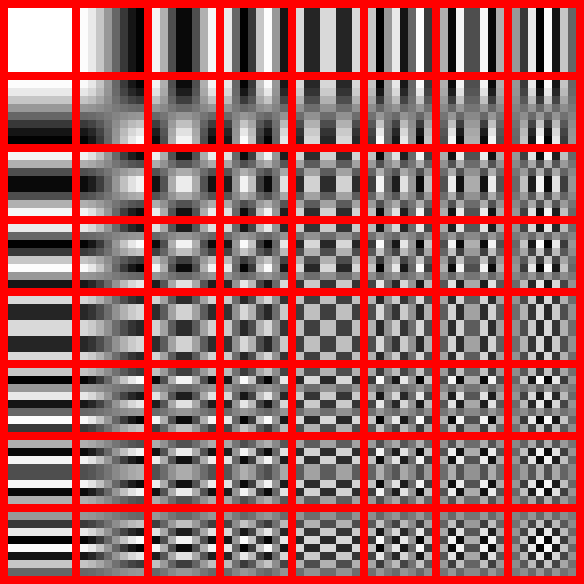
\includegraphics[width = 0.45\textwidth]{img/marco_teorico/Patrones de DCT.png}
            \caption{Patrones de frecuencia para una imagen de 8x8}
            \label{fig:DCT_pattern}
        \end{figure}
    \subsubsection{JPEG}\label{subsubsec: jpeg}
    JPEG es un algoritmo de compresión con la capacidad de disminuir muy significativamente el tamaño de imágenes con pérdidas poco notorias de calidad \cite{jpeg1992}. En general, este algoritmo es bueno en eliminar aquellos elementos que son difíciles de detectar para el ojo humano, privilegiando la luminiscencia por sobre la crominancia cuya detección es menor debido a la concentración de conos y bastones cuya razón es de 6 a 100. Por tanto, la capacidad de reconocer diferencias de brillo y luz es mucho mayor que la de color. Luego los pasos para este algoritmos son:
    
    \subsubsubsection{Conversión del espacio de color}
        En este paso, se cambia el espacio de color desde RGB a YCbCr. Este último se describe como luminescencia, crominancia azul diferenciada y crominancia roja diferenciada. Agrupando de forma efectiva la dimensión perceptiva de los bastones. La fórmula para esta conversión para cada pixel corresponde a:

        \begin{align*}
            \centering
            Y &= 0.299\cdot R + 0.587 \cdot G + 0.114 \cdot B\\
            C_b &= 128 - 0.168736\cdot R - 0.331264 \cdot G + 0.5 \cdot B\\
            C_r &= 128 + 0.5 \cdot R - 0.418688 \cdot G - 0.081312 \cdot B
        \end{align*}

        Esta operación es invertible y no tiene pérdida de información.
        
    \subsubsubsection{Submuestreo de la crominancia}
        En consecuencia de lo mencionado respecto a las características de la visión humana y en el contexto del nuevo espacio de color. Este paso se dedica a submuestrear la información de las imágenes en Cb y Cr a razón de $\frac{1}{4}$ calculando un promedio cada 2x2 pixeles redefiniendo la imagen según estos valores, disminuyendo su tamaño a $\frac{1}{4}$ lo que puede después ser adaptado al tamaño original haciendo upsampling posteriormente para la reconstrucción.
    \subsubsubsection{Transformada de coseno discreta}
        Se aprovecha de la incapacidad del ojo humano para distinguir elementos de alta frecuencia, es decir, aquellos cambios muy rápidos de información entre píxeles para el caso de imágenes. El primer paso corresponde a la división por bloques, en el caso de este algoritmo, son bloques de 8x8 píxeles, cada valor de esta matriz se desplazan del conjunto $[0,256]$ al conjunto $[-128,127]$.\\

        Una vez hecho esto, se genera una matriz de 8x8 donde existen 64 posibles combinaciones de frecuencia según la transformada discreta de coseno en 8x8,es decir, 64 combinaciones base de imágenes de frecuencia. Esta como se mencionó antes es muy útil en términos de concentración de energía. De estas 64 posibilidades se cuenta la cantidad necesaria de cada una para reconstruir la imagen.
    \subsubsubsection{Cuantización}
        Una vez se tiene las repeticiones de frecuencia donde las más altas frecuencias se ubican al extremo derecho. Una matriz de cuantización se aplica, la cual según la calidad de compresión aumentará sus valores de abajo hacia arriba y de derecha a izquierda. A esta división se le busca el entero más cercano, donde naturalmente, aquellas frecuencias altas de menor aparición resultarán nulas y las de menor frecuencia mantendran un valor mayor.
    \subsubsubsection{Longitud de ejecución y codificación Huffman}
        De este resultado, se genera una codificación que recorre toda la imagen de forma serpenteada desde la esquina superior derecha a la inferior izquierda agrupandola en un arreglo. Y con la longitud de ejecución se declara la cantidad de veces que se repite un valor de forma consecutiva en vez de agregarlo esa cantidad de veces.
        

\section{Orden de Morton}\label{sec:morton_order}
    El orden de Morton, también conocido como \textit{Z-order curve}, es una técnica de indexación espacial que permite mapear puntos en un espacio multidimensional (por ejemplo, 2D o 3D) a un valor escalar unidimensional preservando, en la medida de lo posible, la localidad espacial. Fue introducida con el objetivo de mejorar la eficiencia en el acceso secuencial a bases de datos geoespaciales. \cite{morton1966zorder}\\

    La representación tradicional de datos tridimensionales como las nubes de puntos no impone ningún orden explícito sobre los puntos. Sin embargo, muchos algoritmos de compresión, estructuración jerárquica (como octrees) o renderizado acelerado requieren organizar los datos de forma que puntos cercanos en el espacio también estén cercanos en memoria o en disco. El orden de Morton proporciona esta capacidad mediante una codificación binaria de las coordenadas espaciales.
    
    \subsection{Intercalación de bits}
    
    El principio fundamental del orden de Morton es la intercalación de los bits de cada una de las coordenadas espaciales. Dado un punto en el espacio tridimensional con coordenadas enteras \((x, y, z)\), cada coordenada se representa como un entero binario de igual longitud (por ejemplo, 10 bits si el espacio está cuantizado a \(2^{10} = 1024\) unidades por eje).
    
    La clave está en construir un valor escalar \(m\) a partir de los bits de \(x\), \(y\) y \(z\) intercalados de la siguiente manera:
    
    \[
    x = \sum_{i=0}^{b-1} x_i \cdot 2^i, \quad
    y = \sum_{i=0}^{b-1} y_i \cdot 2^i, \quad
    z = \sum_{i=0}^{b-1} z_i \cdot 2^i
    \]
    
    \[
    \Rightarrow \text{Morton code: } 
    m = \sum_{i=0}^{b-1} \left( x_i \cdot 2^{3i} + y_i \cdot 2^{3i + 1} + z_i \cdot 2^{3i + 2} \right)
    \]
    
    En otras palabras, los bits de menor peso de \(x, y, z\) ocupan las posiciones 0, 1, 2 respectivamente en \(m\); los siguientes bits ocupan las posiciones 3, 4, 5; y así sucesivamente. Este procedimiento genera un valor único que se puede utilizar para ordenar o indexar los puntos en memoria.
    
    \subsection{Propiedades}
    
    El orden de Morton tiene las siguientes propiedades fundamentales:
    
    \begin{itemize}
        \item \textbf{Preservación de localidad:} puntos cercanos en el espacio tridimensional tienden a tener códigos Morton similares (aunque no garantiza una vecindad exacta).
        \item \textbf{Jerarquía implícita:} al truncar los bits menos significativos del código Morton, se obtiene una representación de menor resolución del punto, lo que se utiliza en estructuras como octrees.
        \item \textbf{Eficiencia computacional:} la intercalación y desintercalación de bits puede realizarse con operaciones bitwise eficientes, facilitando su implementación en hardware o software optimizado.
    \end{itemize}
    
   En el contexto de esta tesis, el orden de Morton se emplea como mecanismo de indexación para los puntos de la nube durante la partición espacial. Cada punto es convertido a un índice escalar mediante su código Morton, lo que permite realizar una partición espacial coherente en bloques cúbicos jerárquicos, ordenar los puntos para una compresión más eficiente —ya que se agrupan espacialmente en estructuras locales—, y facilitar el acceso jerárquico y progresivo a los datos para tareas como renderizado o reconstrucción. Así, el orden de Morton no solo sirve como herramienta teórica de codificación, sino que actúa como el eje central sobre el cual se organiza la estructura jerárquica de la compresión propuesta.
    
    
    
        

\section{Graph Signal Processing \cite{ortega2022gsp}} \label{sec: gsp}
    \subsection{Notación y conceptos básicos de grafos}

    % Primeramente, cabe destacar la notación recurrente al trabajar con grafos. Dado que estos corresponden a una red interconectada de puntos que pueden representar diversas cosas se define su estructura más elemental de la siguiente manera.

    Se define la estructura más elemental de grafos de la siguiente manera:

    \begin{itemize}
        \item \textbf{Nodos o vértices}: corresponden a los puntos de conexión y pueden representar casi cualquier cosa (puntos en el espacio, puntos en el tiempo, procesos, etc.). Se denotan como $\mathcal{V} = \{v_1,v_2,...,v_n\}$.
        \item \textbf{Aristas}: denotan la conexión entre dos vértices. Pueden ser direccionados o no direccionados. Se denotan como $\mathcal{E} = \{e_1,e_2,...,e_m\}$. A veces se denota como $e_{ij} = v_i v_j$, implicando que es la arista que conecta el nodo $i$ con el nodo $j$. En caso de ser direccionadas, decimos que $e_{ij} \neq e_{ji}$. Para las no direccionadas, se cumple que $e_{ij} = e_{ji}$.
        \item \textbf{Pesos}: los ponderadores asociados a cada arista. Estos valores tienen dos perspectivas: la de \textit{distancia}, donde un mayor valor indica menor conexión, y la de \textit{similitud}, donde un mayor valor indica mayor similitud. Se denota el conjunto de todos los pesos desde un nodo como: $\mathcal{W}_i = \{w_{ij}, \; \forall j \; | \; e_{ij} \in \mathcal{E}_i \}$.
        \item \textbf{Dirección}: como se mencionó, las aristas pueden o no tener un sentido, es decir, la conexión se realiza con una orientación particular de un nodo a otro o no. En este último caso, la relación es totalmente recíproca y equivalente. Esto clasifica a los grafos en dos tipos: \textit{directos}, que implican pesos distintos y/o conexiones no permitidas, e \textit{indirectos}, cuyos pesos son iguales y las conexiones son en ambos sentidos.
    \end{itemize}

    Desde la perspectiva de grafos en el análisis de señales, se entiende que para cada nodo en $\mathcal{V}$ existe un escalar o un conjunto de escalares que representan un valor de señal. Esta señal puede cambiar en el tiempo o ser estática, todo dependerá de la construcción y el significado del grafo. %Naturalmente, si se construye este paradigma de señales en contexto de grafos se deben trasladar e interpretar los conceptos típicos de señales y procesamiento de señales.\\
    
    Cada grafo está estructural y funcionalmente descrito por estructuras algebraicas simples. En primer lugar tendremos la matriz de adyacencia ($A$), que resume las aristas y pesos en una sola matriz con toda la información del grafo. Sea $a_{ij}$ el elemento $i$,$j$ de la matriz de adyacencia:

    \begin{equation*}
        a_{ij} = w_{ij} \quad \quad \forall (i,j) \in \mathcal{E}    
    \end{equation*}

    \vspace{0.4cm}

    Luego, existe la matriz de grado ($D$) que describe el \textit{grado de conectividad} de cada nodo. Esta será una matriz diagonal, donde cada elemento $d_{ii}$ corresponderá a la suma de los pesos de todas las conexiones del nodo $v_i$.

    \vspace{0.4cm}

    \begin{equation*}
        d_{ii} = \sum_{j}a_{ij}
    \end{equation*}

    \vspace{0.4cm}
    
    Con estos dos elementos, podemos resumir el contenido estructural del grafo en la matriz laplaciana ($L$). Esta matriz se construye a partir de la operación simple de la matriz de grado y la matriz de adyacencia.

    \begin{equation*}
        L = D- A
    \end{equation*}
    
    \vspace{0.4cm}
    
    Adicionalmente, los grafos pueden poseer \textit{self-loops}, es decir, conexiones de nodos hacia sí mismos. En general estos elementos tienen un efecto relevante en las transformadas que se explicarán posteriormente. Matemáticamente un \textit{self-loop} se describe como una arista $e_{ii}$ que conecta un nodo sobre si mismo con un peso $w_{ii}$. Para describir el efecto de éste se introduce el laplaciano generalizado:

    \begin{equation*}
        L_g = C + D - A \quad \quad C = diag(a_{11},a_{22},...,a_{nn})
    \end{equation*}

    \vspace{0.4cm}
    
    Describiendo lo anterior, tendremos completamente representada la estructura del grafo en una sola expresión algebraica. A partir de ella, podremos procesar las señales involucrando. %la información de señal con la información impuesta por su estructura.
    
% Transformada 
\subsection{Transformada Gráfica de Fourier}\label{subsec: gft}

    GFT (\textit{graph fourier transform}) es una transformada ortogonal generada a través de los vectores propios ordenados del laplaciano generalizado. Es decir sean $\{ \phi_1, \phi_2, ..., \phi_n \}$ los vectores propios considerando los valores propios $\lambda_1 \leq \lambda_2 \leq ... \leq \lambda_n$ diremos que:

        \begin{equation*}
            U = [\phi_1, \phi_2, ..., \phi_n] \Longrightarrow GFT = U^T
        \end{equation*}

    Lo que representa una transformada sin pérdida de información, es decir, la señal transformada al dominio espectral de grafo puede ser reconstruida completamente. Sea $x$ la señal original de tamaño $(N,1)$ y $\hat{x}$ los coeficientes transformados de tamaño $(N,1)$. Así, la operación realizada por la transformada se ve de la siguiente manera:

        \begin{equation*}
            \hat{x} = U^Tx \quad \quad x = U\hat{x}
        \end{equation*}

    \vspace{0.4cm} 
    
    Esto implica que ambos espacios son ortogonales al igual que la transformada clásica de Fourier, lo que es visible matemáticamente al notar que:
        \begin{equation*}
            U^T U = I
        \end{equation*} 

    \vspace{0.4cm}
    
    Los valores descritos por $\hat{x} = [\hat{x}_1,\hat{x}_2, ..., \hat{x}_n]$ representan los \textbf{coeficientes transformados} y separan la frecuencia de manera similar a como lo haría la transformada de Fourier clásica por componentes de la siguiente manera:

    \begin{equation*}
        \hat{x}_i \cdot \phi_i = f_i \quad \quad x = \sum_{i=1}^N f_i = \sum_{i=1}^N \hat{x}_i \cdot \phi_i 
    \end{equation*}

    Entendiendo esto, podemos hacer reconstrucciones parciales de la señal, perdiendo parte de su información, pero mostrando su comportamiento general y relevante para analizarla e interpretarla. Para toda señal podremos construir un conjunto $M \subset \{1,2,...,N\}$ tal que:

    \begin{equation*}
        x_M = \sum_{i \in M} f_i
    \end{equation*}

    \vspace{0.4cm}

    Para evaluar la información perdida podremos siempre comparar las reconstrucciones con la señal original, para conocer qué tan representativas son las $|M|$ bases. Por ejemplo, se puede hacer un análisis para distintos conjuntos $M$ comparando la señal según la raíz del error cuadrático medio de la reconstrucción:

    \begin{equation*}
        RMSE(x_M, x) = \sqrt{\frac{\sum_{i=1}^N{\left(x_M(i) - x(i)\right)^2}}{N}}
    \end{equation*}

    
\section{Rate-Distorsion Theory}\label{sec: rdt}
    La teoría de tasa distorsión es una de las muchas derivadas de la teoría de Shannon y la codificación de fuentes. El concepto es aprovechar de la mayor manera posible la redundancia de la fuente sujeto a un criterio de fidelidad. En otras palabras, el objetivo de esta teoría es la representación de la fuente con el menor número de bits posibles (tasa) para una dada calidad de reproducción (distorsión) \cite{ortega1998rate}. \\

    Una reflexión previa relevante para estos métodos es que así como las distintas metodologías de compresión pueden diferir mucho en efectividad según el tipo de dato, también pueden diferir entre muestras. Es por tanto otro objetivo de esta teoría aprovechar lo mejor de ambos mundos, primero utilizando la información muestra a muestra para encontrar los mejores parámetros de compresión como también aprovechar la eventual correlación entre muestras subsecuentes. \\

    Otra mención relevante, es que estos métodos solo hacen sentido en un contexto donde exista un escenario de ganancia-pérdida lo que hace matemáticamente relevante un proceso de optimización. En ese sentido, esta teoría es aplicable para métodos de compresión con pérdida de información, donde la pregunta es; cuánta fidelidad de representación se está dispuesto a perder para reducir el almacenamiento necesario para la fuente o sus indicaciones de transmisión.

    \subsection{Métricas de distorsión}
        Ahora, la definición de la métrica de distorsión no es una discusión trivial, en tanto es relevante considerar una combinación de variables cuantitativas y cualitativas. Es decir, es especialmente relevante para datos que dependen de la percepción del consumidor o usuario, en la mayoría de las casos un humano. En resumen, las métricas deben buscar una correlación con el impacto perceptivo del sujeto.\\

        Sin embargo, lo anterior lleva a otra discusión respecto a la generalidad del método, ya que considerar las diferencias individuales de cada sujeto es impracticable. Este objetivo se ha demostrado complejo de resolver, mas a través del conocimiento especializado, por ejemplo en la percepción del color en tanto su resolución biológica (conos y bastones) o el audio según la capacidad humana de escuchar cierto rango de frecuencias.\\

        Mezclando lo anterior con el error mínimo cuadrado, existe una ponderación perceptual conjunta con una métrica cuantitativa para dimensionar la distorsión de los métodos de compresión con pérdida. Un buen ejemplo, observando lo mencionado anteriormente en JPEG es, en el espacio transformado, enfocar el error en la percepción humana enfocandose matemáticamente en el canal de luminiscencia. Por ejemplo, considerando la distorsión como:

        \begin{equation}
            \mathrm{RMSE}(Y, q) = \frac{1}{\sqrt{n}} \left\| Y - q^{-1}(q(Y)) \right\|_2
        \label{eq: rmse_dist}
        \end{equation}
            
    \subsection{Optimización en sistema concreto}
        Si bien existe una discusión teórica sobre cual es el espacio de optimización y el mejor desempeño en tasa distorsión sin restricciones. La presente investigación se centra en la propuesta de un esquema de codificación que limita la optimización a un sistema específico. Este se puede considerar que captura la relevancia estadística y las dependencias asociadas a la fuente, por tanto, el proceso de optimización se centrará en el mejor punto de operación para un esquema ya no abstracto, sino concreto.\\

        Como se mencionó anteriormente en esta sección, considerando el paradigma analizado anteriormente de codificación basado en transformadas, estamos en un esquema bien definido que cumple con los requisitos descritos anteriormente. Desde ese escenario existen multiplicidad de métodos bien estudiados de optimización tasa-distorsión.

        Es relevante mencionar, que lo anterior también incluiría el conocimiento del decodificador, ya que no considerar la información necesaria para la recuperación de la fuente y la calidad de la fuente recuperada, sería miope para el análisis de tasa-distorsión.\\

        Por lo tanto, estaremos en presencia de un espacio de optimización tasa-distorsión discreto para una tipo de entrada específica. Luego el objetivo es: "Dado un entorno de codificación donde el decodificador es completamente definido, optimizar la codificación de una secuencia particular de imagen tal que cumpla algunos objectivos tasa-distorsión"\cite{ortega1998rate}\\

        Para esta tarea, existen dos elementos relevantes a considerar según la aplicación final esperada para la metodología planteada. Primero, está la complejidad, donde será importante diferenciar entre métodos pensados en tiempo real y aquellos que no lo son. En este último caso, la complejidad siempre que los recursos computacionales lo permitan, no está limitada y se pueden realizar multitud de operaciones a diferencia de una propuesta en tiempo real. Segundo, está la definición de la función de costo donde el diseño debe considerar la prioridad, la ponderación y la escala de los elementos a minimizar y como estos afectan el resultado final. Ya que, como se mencionó anteriormente, existe una relevancia de la percepción no es lo mismo optimizar para un resultado local que para un resultado globalmente óptimo.\\

        \subsubsection{Restricciones de almacenamiento posible}
            En distintos contextos, la optimización de nuestro método puede estar restringido por condiciones físicas de almacenamiento o una tasa de referencia a superar. Por ejemplo, el espacio restante en disco puede limitar las elecciones de parámetros del método. Sea $x(i)$ un punto de operación para una secuencia de código $i$ y $R_T$ una restricción general de memoria. Podemos expresar esto tal que:

            \begin{equation}
                \sum_{i=1}^{N} r_{ix(i)} \leq R_T
            \end{equation}

            o de manera local, siendo $r_t$ una restricción de referencia:

            \begin{equation}
                r_{ix(i)} \leq r_t
             \end{equation}
            Además de alguna métrica $f_i$, $f$ que debe ser minimizada local o globalmente respectivamente.\\

            Este consideracón del almacenamiento posible o de restricción de tasa obliga a considerar no tan solo la métrica de distorsión como la discutida en \ref{eq: rmse_dist} sino también la tasa. Para incluir esta restricción el paradigma más clásico y utilizado ampliamente en el contexto de compresión es la optimización Lagrangiana. Básicamente, se introduce un multiplicador de Lagrange $\lambda \geq 0$ y una función de costo de Lagrange tal que:

            \begin{equation}\label{eq: rdo_lagrange}
                J_{g}(\lambda) = d_{ij} + \lambda \cdot r_{ij}
            \end{equation}

            Donde $d_{ij}$ corresponde a la distorsión para el índice de cuantización $j$ (cierto paso de cuantización) y $r_{ij}$ corresponde a la tasa o tamaño del código que representa dicha información cuantizada. Con esto podemos controlar la relevancia que damos a la tasa en el proceso de optimización minimizando local o globalmente la función objetivo. \\

            Finalmente, hay una cuestión relevante que surge de este análisis respecto a como obtenemos métricas precisas para optimizar resultados en un proceso que no es determinístico. Por ejemplo, al ocupar codificación entrópica, este es un método estadístico y probabilístico que no es independiente de la distribución de los coeficientes transformados. Es por tanto recurrente la utilización de aproximaciones de la tasa, basadas en la compresión específica de la codificación a utilizar y esto es algo que se debe abordar al desarrollar un método de compresión.


